\subsection{Clustering}
    Given: $X = \{x_1, x_2, ..., x_n\} \in \mathbb{R}^d$\\
    \begin{tabular}{m{0.4\linewidth} | m{0.54\linewidth}}
        Initialize $K$ centroids (randomly): $z_i \in \mathbb{R}^d$ $\rightarrow Z = \{z_1, z_2, ..., z_K\}$ & \begin{minipage}{\linewidth}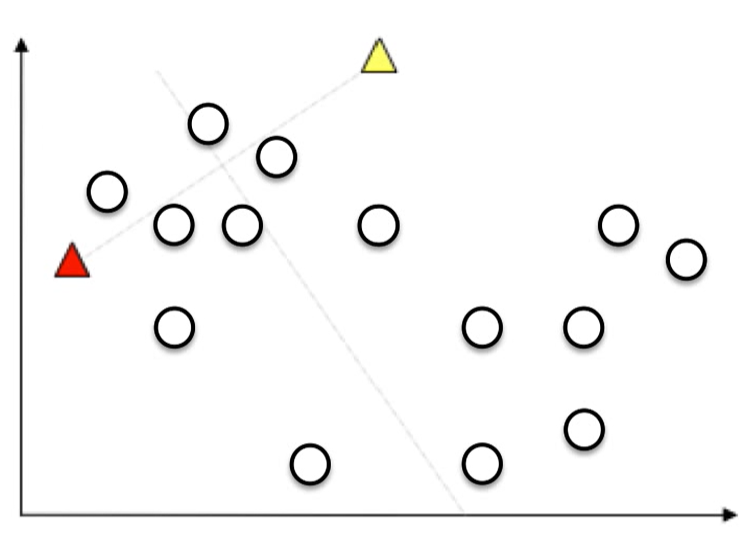
\includegraphics[width = \linewidth]{src/8_ml/images/cluster_centroid_placing.png}\end{minipage}\\
        \hline
        Assign each point to centroid it is closest to:
        \begin{align*}
            c(x) = \text{argmin}||x - Z_i||
        \end{align*}
        & 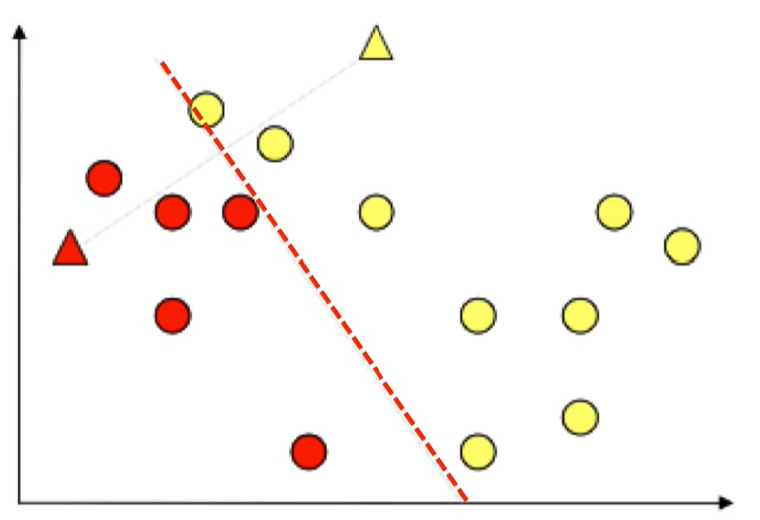
\includegraphics[width = \linewidth]{src/8_ml/images/cluster_assign_points.png}\\
        \hline
        Place centroid in the mean of its assigned points:
        \begin{align*}
            S_j = x_i \in z_j\\
            z_j = \frac{1}{len(S_j)} \sum_{S_j} x
        \end{align*}    
        & \begin{minipage}{\linewidth}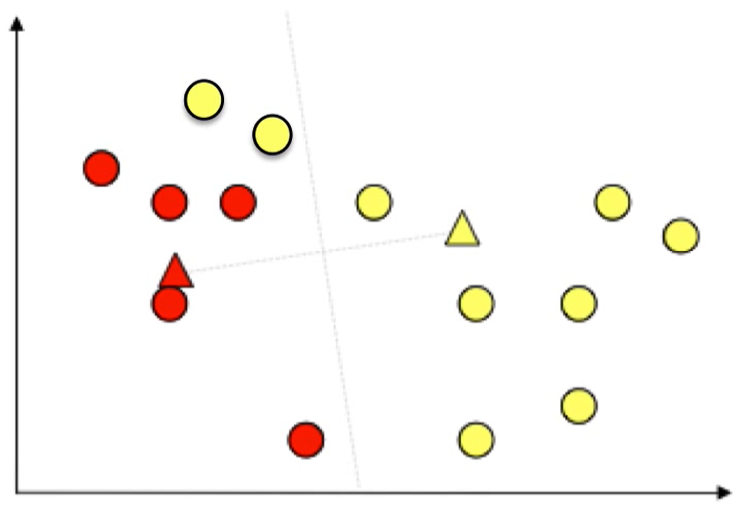
\includegraphics[width = \linewidth]{src/8_ml/images/cluster_move_centroids.png}\end{minipage}\\
    \end{tabular}

    Repeat step 2 and 3 until the centroids have converged, that means no point is assigned to another centroid anymore\\
    Overfitting: Each point has its own centroid\\
    Loss function:
    \begin{align*}
        L = (\sum ||x_i - z_{x_i}||^2) + \lambda e^K
    \end{align*}
    squared distance of point to its centroid + penalty for using to many centroids (prevents overfitting)